\documentclass[]{article}
\usepackage{lmodern}
\usepackage{amssymb,amsmath}
\usepackage{ifxetex,ifluatex}
\usepackage{fixltx2e} % provides \textsubscript
\ifnum 0\ifxetex 1\fi\ifluatex 1\fi=0 % if pdftex
  \usepackage[T1]{fontenc}
  \usepackage[utf8]{inputenc}
\else % if luatex or xelatex
  \ifxetex
    \usepackage{mathspec}
  \else
    \usepackage{fontspec}
  \fi
  \defaultfontfeatures{Ligatures=TeX,Scale=MatchLowercase}
\fi
% use upquote if available, for straight quotes in verbatim environments
\IfFileExists{upquote.sty}{\usepackage{upquote}}{}
% use microtype if available
\IfFileExists{microtype.sty}{%
\usepackage{microtype}
\UseMicrotypeSet[protrusion]{basicmath} % disable protrusion for tt fonts
}{}
\usepackage[margin=1in]{geometry}
\usepackage{hyperref}
\hypersetup{unicode=true,
            pdftitle={dissertation\_writeup\_draft},
            pdfauthor={Alassane Ndour},
            pdfborder={0 0 0},
            breaklinks=true}
\urlstyle{same}  % don't use monospace font for urls
\usepackage{graphicx,grffile}
\makeatletter
\def\maxwidth{\ifdim\Gin@nat@width>\linewidth\linewidth\else\Gin@nat@width\fi}
\def\maxheight{\ifdim\Gin@nat@height>\textheight\textheight\else\Gin@nat@height\fi}
\makeatother
% Scale images if necessary, so that they will not overflow the page
% margins by default, and it is still possible to overwrite the defaults
% using explicit options in \includegraphics[width, height, ...]{}
\setkeys{Gin}{width=\maxwidth,height=\maxheight,keepaspectratio}
\IfFileExists{parskip.sty}{%
\usepackage{parskip}
}{% else
\setlength{\parindent}{0pt}
\setlength{\parskip}{6pt plus 2pt minus 1pt}
}
\setlength{\emergencystretch}{3em}  % prevent overfull lines
\providecommand{\tightlist}{%
  \setlength{\itemsep}{0pt}\setlength{\parskip}{0pt}}
\setcounter{secnumdepth}{5}
% Redefines (sub)paragraphs to behave more like sections
\ifx\paragraph\undefined\else
\let\oldparagraph\paragraph
\renewcommand{\paragraph}[1]{\oldparagraph{#1}\mbox{}}
\fi
\ifx\subparagraph\undefined\else
\let\oldsubparagraph\subparagraph
\renewcommand{\subparagraph}[1]{\oldsubparagraph{#1}\mbox{}}
\fi

%%% Use protect on footnotes to avoid problems with footnotes in titles
\let\rmarkdownfootnote\footnote%
\def\footnote{\protect\rmarkdownfootnote}

%%% Change title format to be more compact
\usepackage{titling}

% Create subtitle command for use in maketitle
\providecommand{\subtitle}[1]{
  \posttitle{
    \begin{center}\large#1\end{center}
    }
}

\setlength{\droptitle}{-2em}

  \title{dissertation\_writeup\_draft}
    \pretitle{\vspace{\droptitle}\centering\huge}
  \posttitle{\par}
    \author{Alassane Ndour}
    \preauthor{\centering\large\emph}
  \postauthor{\par}
      \predate{\centering\large\emph}
  \postdate{\par}
    \date{23/08/2019}


\begin{document}
\maketitle

\hypertarget{introduction-and-objectives}{%
\section{Introduction and
Objectives}\label{introduction-and-objectives}}

\hypertarget{background-to-the-problem-choice-of-project-and-beneficiaries}{%
\subsection{Background to the problem, Choice of project and
beneficiaries}\label{background-to-the-problem-choice-of-project-and-beneficiaries}}

Growth model selection is a large literature in many domains which often
takes into account the specificity of the subject matter. For instance,
in biostatistics, bioassay data can be modeled using different logistic
like functions (e.g.~4PL or 5PL) {[}CITATION{]} that are tested against
each other. Generally, model selection is a basic scientific requirement
that answers what functional form a set of data corresponds to. There
are differrent requirements for a function to be chosen in a selection
problem such as the simplicity of the model (Occramm's razor states that
the simpler model should prevail), the estimation of parameters or even
the ``certainty'' of the selection. For instance, in economics different
models can be tested against each other to verify how well they explain
GDP growth{[}CITATION{]}. In such a case, the main requirement of the
models is interpretability as it is required for policy making. In
contrast, for prediction interpretability of neural nets for example is
not always necessary. Naturally, depending on the use case, it is
crucial to select the best functional form as the real one is often
unknown, and a wrong selection invalidates any following inference
(Nguimkeu, 2014).

Most domains use statistical foundation to select models. It is often
done comparing the relative likelihood that the data's underlying
generating process was given by a model{[}CITATION{]}. This is a well
known and documented problem. However, there is a specific context that
is not tackled often by the current literature : if one were to classify
a large pool of different datasets according to the functional form each
one of them follows given a set of known functional forms, how would one
go about it? This classification problem was posed here by our
commercial partner and is the subject of matter. Therefore, by comparing
several relevant model selection strategies, this project aims to obtain
a growth model classification method that by construction classifies
datasets accurately but also demonstrates the uncertainty level by which
it is doing so and provides the estimated parameters.

The project was chosen for its application in a wide variety of domains
as well as its relevance for the specific use case brought forth by our
commercial partner. This analysis will therefore aim to contribute to
the literature of model selection by offering an experimental evaluation
of several model selection processes. Furthermore,it can also be used as
a base for the commercial partner's model evaluation.

\begin{itemize}
\tightlist
\item
  {[}IF TIME PERMITS{]} Contribution to literature as unexplored method
  - combination of Bayes factor and Harris paper
\end{itemize}

\hypertarget{objectives-metrics-and-broad-methods}{%
\subsection{Objectives, metrics and broad
methods}\label{objectives-metrics-and-broad-methods}}

The aim of the project is to construct a dataset classification method
that can accurately identify the functional form the dataset is
following. The challenge of this task arises when the dataset to be
classified is noisy and the ratio of signal to noise weakens.
Consequently, it is essential for the classification to be able to
detect any underlying patterns in a noisy setting. Thus a large part of
the study will focus on how well the classification performs as the
noise increases. Ideally, the classifier will can quantify the noise
level for a given dataset. Furethermore, our model should offer an
estimation that identifies its classification ``certainty'' and an
estimation of the parameters of the model. Finally, as the selection
process must scale to a large amount of datasets, we record the
computation cost of each method and will favour a less expensive but
accurate classifier.

Section {[}methodology{]} provides more details on the methodology used.
Here we offer a brief overview of the ways the classification task was
handled. There are broadly speaking two ways of thinking of how one
might choose a model: a frequentist one which aims to compute a
statistic on the data for which we know the distribution {[}citation{]}
and a Bayesian approach which compares the posterior of different models
using methods such as Bayes factor. Here we apply both views on a
generated dataset and compare using the criteria described above.

\begin{itemize}
\tightlist
\item
  Furthermore, there have been interesting developments in combining
  Bayesian methods and cross validation as they are not mutually
  exclusive methods and can contribute to robust estimates. Such works
  include Bürkner et al. (2019) where the authors aim to improve upon
  leave-future-out cross-validation (LFO-CV) - an adaptation of
  leave-one-out cross-validation (LOO-CV) to timeseries - to reduce
  computation time.
\end{itemize}

\hypertarget{context-and-relevant-literature}{%
\section{Context and relevant
literature}\label{context-and-relevant-literature}}

The analysis carried out in this project has two fundamental building
blocks which are data simulation and model selection strategies. For
this reason relevant literature on both these topics will be presented
in this section.

\hypertarget{data-simulation-contextual-elements}{%
\subsection{Data simulation contextual
elements}\label{data-simulation-contextual-elements}}

Data simulation simply refers to the process of generating random
numbers from a distributional statements. It a common statistical
technique to understand or forecast phenomenons that might occur in
observational data, all so in a controlled context. Kery and Royle
(2016) provide an insightful outline of the advantages of simulations.
Here we highlight some of them as these were the principle reasons for
simulations used in this study. According to them data simulations allow
researchers to know the truth behind the data, in a parametric context
for instance. This is partucularly important as the researcher has less
insight on the internals of certain black box algorithms. The authors
point out that having knowledge of parametric values before applying a
Markov-Chain Monte Carlo (MCMC) simulation as is done in the present
study, is necessary as it confirms that the simulation is not going
astray. Additionally, it can be noted that MCMC by nature is a
simulation and represents a corner stone of Bayesian statistical
techniques (Gelman) therr gain emphasizing its importance. Kery and
Royle (2016) also highlight that simulations help calibrate model
parameters. More generally, it can added that simulations have also been
used in order to study, compare and contrast particular models in many
fields. For instance in Ploeg et al (2014), the authors study the effect
of small sample size on different modelling techniques in patient
survival rates; the data they use was simulated based on observed data.
In Murari et al. (2019) the authors compare different information
criteron in model selection problems using simulations. These examples
not only show that simulation is present in many domains but also serves
as a solid control to study intra and inter model specificities.
Finally, Kery and Royle (2016) also point out that simulations allow
researchers to include errors that can then be accounted for and studied
as one should do with obersved phenomenon. This principle is important
in our context and can be illustrated by Harris (2015) who use Bayesian
techniques to account for sampling errors in a simulated dataset.

Although, simulation is undeniably an important and effective tool in
the researchers aresenal, it must be noted that there exist different
forms of data simulations. Since this research project originally stems
from biological literature, examples in biology and biostatistics will
be emphasized here. Broadly speaking simulation methods can be divided
between Simulation Optimization methods and algebraic methods as
described by Amaran et al (2015). The former refers to techniques used
to optimize stochastic simulations that cannot be described
algebraically. These are more black-box type simulations and can be
found in projects such as Montagna et al (2015) which proposes a
framework to optimise parameters in biological system development
simulations. It can be stated that these models are very powerful in
very specific settings anc can lack generalisation as pointed out by Fu
et al (2000). In contrast algebraic solutions are more general but it
cannot explicitly tackle more precise stochastic tasks. For instance, we
know that population growth in ecological studies follows a logistic
growth process (Brimlow et al. - 2013). This is a general result and
observed data can be seen to fit this pattern as demonstrated when
Buehler et al. (1991) adapt logistic growth functions to take into
account the human activity impoact on the bald eagle population in the
US. However, to model stochastic differential equations as is necessary
in the seperation of DNA molecules (Cho and Dorfman - 2010), stochastic
simulations are necessary. In this study since generalisation was
necessary the algebraic route described in section
\protect\hyperlink{data}{Data} was taken.

CAN USE Sigman (2010) for inverse transform method to create data and
can discuss tools in python -
\url{https://www.biorxiv.org/content/biorxiv/early/2017/12/21/088773.full.pdf}
- Morpheus and CompuCell3D - logistic regression for shape of population
: QuantitativeConservationBiology -
\url{https://www.nature.com/scitable/knowledge/library/an-introduction-to-population-growth-84225544/}
-
\url{https://www.sciencedirect.com/science/article/pii/S0888754383711808}
* Ed Harris

\hypertarget{model-selection-contextual-elements}{%
\subsection{Model selection contextual
elements}\label{model-selection-contextual-elements}}

The second building block of this research is statistical model
selection which refers to the the step of selecting the most appropriote
statistical model among a set of candidates for a given dataset (Ding et
al - 2018). This can be diffentiating the number of regressors usind in
a linear regression or selection the type of neural network to use. This
step is performed in an array of domains: in ecological science where
researchers use mark-recapture (marking an animal and recapturing in a
latter period) in order to estimate the population and survavability
probabilities of a species they make multiple statistical models compete
and use the best for inference (Johnson et al - 2004); in cosmology,
researchers make models whose parameters have been estimated compete to
describe phenomenons such as the geometry of the expansion of the
universe (Liddle et al. - 2006). Therefore the overarching importance of
model selection is not contested; as pointed out by a Nguimkeu (2014) a
wrong statistical selection invalidates any following inference. In
addition to selection, as pointed out by Claeskens and Lid Hjort (2010),
model averaging is a closely linked problem as researchers might wish to
combine relevant competing models. Even though model selection's value
is not contested it remains an open problem in statistics that often
requires the combination of multiple methods. Furthermore, within the
literature there are different ways of approaching the selection
problem. Dormann (2018) outlines the schools of thought that are
prevalent in model selection and averaging issues. This discussion is
very relevant to understand and compare the different paths available.

On one hand, empirisits base model selection on the data. Their methods
have proven effective and are extensively present in the machine
learning literature {[}citation{]}. Popular methods in this line of
thought include selection using algorithms such as cross validation
(Allen, 1974; Stone, 1974; Geisser, 1975) or bootstrp aggregations.
These methods are often computationally more expensive than others but
have proven very effective (Dormann - 2018) leading them to have
prominent supporters such as Lambert (2018) or Bishop (). In general the
algorithms in this school of thought repeatidly and consitently sample
data points and then compute an average metric based on the samples or
use more brute force methods such as grid searches. {[}PLAN AND
FINISH{]}

Intro : * what is model selection, why is it useful? * link to model
averaging - Claeskens and Lid Hjort (2010) + Dormann (2018) * 3 types of
model selection frameworks : - Empirical methods : Cross validation -
Information Criterion - Bayesian model selection -combining these
methods

\begin{itemize}
\tightlist
\item
  LOO-CV
\item
  Bayesian books
\item
  Bürkner et al. (2019)
\item
  Claeskens and Lid Hjort (2010) (Model selection)
\end{itemize}

\hypertarget{data}{%
\section{Data}\label{data}}

The data used in this project was generated data. There are several
practical and methodological reasons for doing so. First,
methodogically, generating data makes sense: as advised by Kéry and
Royle (2016) as this offers a ideal control environment under which
parameters and hyper-parameters are known. Furthermore, in growth cell
literature, from which this project stems (e.g.~Harris et al. (2016))
synthetic data is standard practice. Second, data from the commercial
partner that was meant was to be analysed here was unavailable due to
legal restrictions and no open source equivalents were found. As the
synthetic data is at the heart of the analysis this section will
describe in greater detail the data meant to be mimicked and the process
and tools used to do so.

The type of generated process in this project is similar to a cell
counting process proposed by Morpheus or CompuCell3d with certain
restrictions posed by the commercial partner's contextextual information
which led to custom data generation. The restrictions posed by the
commercial partner were as follows :

At any time \(x\) we must be able to estimate the number of a given cell
count. We have knowledge of the growth function that the cells take
(i.e. \(f(x)\)). We also know that introducing an agent in our cell
sample alters the growth path that the sample follows to another process
(say \(g(x)\)). Given this information, we should be able to obtain the
number of cells for any given time on the condition that we have
knowledge of the presence or absence of the agent. However, if we do not
know if the agent has been introduced in the sample then we must choose
whether we estimate the numbers of cells using \(f(x)\) or \(g(x)\)
based on the count. At this point, a simple model selection is
sufficient to capture the correct model or even combine the two models
if necessary. However, the primary difficulty with this is that the
counting process is subejct to a large amount of noise. Therefore, the
problem at hand is to find the ideal model selection method under noisy
conditions. In this case, the ideal model selection would favour a
growth function that is able to identify the true growth process along
with the corresponding parameters. Furthermore, it is interesting for
the researcher to be able to jauge the uncertainty surrounding the
selected model and its parameters. Note that the growth functions
(\(f(x)\) and \(g(x)\)) were not avaible and we therefore made simple
assumptions to create them.

Within this context, the data generated was meant to mimic a growth
process through time in which \(x\) represents the time through which
the count \(y\) increases. To bound the problem the count was generated
and then normalized (min-max normalization). Therefore we have :

\[x \sim U(0, 1000)\] \[y \in[0, 1]\] Although the normalization is
clearly not realistic, it is ideal to bound the problem and does not
undermine generalisation.

The two growth functions used to generate the data were a simple linear
function (1) and a logistic function (2) of the following forms :

\begin{enumerate}
\def\labelenumi{(\arabic{enumi})}
\tightlist
\item
  \(f(x) = \alpha + \beta \times x\)
\end{enumerate}

where \(\alpha\) is the intercept and \(\beta\) the the coefficient of
\(x\) and :

\begin{enumerate}
\def\labelenumi{(\arabic{enumi})}
\setcounter{enumi}{1}
\tightlist
\item
  \(g(x) = \frac {L} {1 + e^ {(-k(x - x0))}}\)
\end{enumerate}

where \(L\) describes the maximum value the curve could take, \(k\)
describes the growth rate of the logistic function and \(x0\) represents
the sigmoid's midpoint.

For all these parameters, the following values were uniformly drawn :

\begin{itemize}
\tightlist
\item
  \(\alpha \sim U(0, 0.05)\)
\item
  \(\beta \sim U(0,0.2)\)
\item
  \(L \sim U(0.9, 1.1)\)
\item
  \(x0 \sim U(\frac{max(x)}{4} , \frac {3max(x)}{4})\)
\item
  \(k \sim U(0.5, 2)\)
\end{itemize}

In order to simulate the noise in the problem and analyze it in a
coherent manner different levels of additive Gaussian errors were
introduced. The Gaussian errors all had a mean of 0 and a a variance
\(\sigma\) ranging from 0.1 to 1 by intervals of 0.1. In the following
discussion we refer to each of these noise levels as noise buckets. Each
noise bucket was comprised of 100 synthetic datasets. To generate the
data, custom \texttt{numpy} based functions were created and caleld. The
meta-data regarding the created dataset was stored along with the data
in nested \texttt{pandas} dataframes.

\begin{figure}

{\centering \includegraphics[width=1\linewidth]{/Users/andour/Google Drive/projects/Dissertation/Final figures/data_sample_table} 

}

\caption{Sample of data used in tabular format}\label{fig:unnamed-chunk-1}
\end{figure}

To understand the robustness of any of the selection processes used, we
add to the generated data a drift which distorts the growth functional.
The drift was added to a rescaled dataset and and was unifomly
distributed \(drift \sim U[0.5, 1]\). From the synthtic data we record
the x and y values (which are reffered to as the datasets) as well as
the label (i.e. ``linear'' or ``logistic''), the set of corresponding
parameters and the associated noise bucket. A subset of the data used is
presented in figure \ldots{} to provide clarity on the data used.

\begin{figure}

{\centering \includegraphics[width=1\linewidth]{/Users/andour/Google Drive/projects/Dissertation/Final figures/data_samples} 

}

\caption{As noise increases the underlying process becomes harder to spot}\label{fig:unnamed-chunk-2}
\end{figure}

To clarify the problem we face in the selection process, figure \ldots{}
illustrates the distortion that occurs as we increase the noise in the
data. The grphic on the left shows very little noise (smallest noise
bucket in the data). Here one could easily eyeball the functional form
associated to each dataset. However, the figure on the right
demonstrates that as we add noise in the data this task becomes less
evident and requires a methodological selection process.

\hypertarget{methods}{%
\section{Methods}\label{methods}}

This section describes the different estimation strategies used for
model selection. To compare how well the different methods performed, we
look at how well the datasets are classified as well as how confident
the method is in the classification. Furthermore, as the systematic
error and the parameters are of interest, we also focus on the estimated
parameter values for different noise levels as well as the estimation of
the error itself when possible. Finally, the time/complexity required
for the estimation is also an important aspect of the study. To
structure this discussion we first focus on selection strategies that
are more often regarded as Frequentist methods {[}describe more{]} and
then we highlight Bayesian model selection processes.

\hypertarget{frequentist-model-selection}{%
\subsection{Frequentist model
selection}\label{frequentist-model-selection}}

As discussed in section \ldots{} there are a battery of different
methods to perform model selection, some of which shall be used in this
study. However, before performing any selection it is important to
estimate our models. Fitting the models to the data or curve fitting
refers to the process of obtaining a mathematical function that can
approxite a data. There are many approches to solve such a problem but a
common one is to solve the least square problem shown in formally shown
equation.

\[\min_{\theta} \sum_{n=1}^{N} (y_n - \hat y(\theta,x))^2\] where
\(y(\theta,x)\) is \(f(x, \theta)\) or \(g(x, \theta)\) depending on the
functional form chosen and \(\theta\) is the vector of parameters. Least
square aims at minimizing the sum of the distances between the fitted
curve and the data points. Here a noticable difference has to be noted
between a linear functional form and a logistic one: The former
represents an unbound problem whereas the logistic function is by
contruction bounded. This implies that different algorithms must be used
in order to solve apply curve fitting to the two functions.

\begin{itemize}
\item
  \begin{enumerate}
  \def\labelenumi{(\roman{enumi})}
  \tightlist
  \item
    Solving the linear least square problem : Solving the linear
    regression problem is straightforward and a commmon result. As such
    the details of solving it are not expanded on here. If needed,
    readers can refer to {[}add reference{]}.
  \end{enumerate}
\item
  \begin{enumerate}
  \def\labelenumi{(\roman{enumi})}
  \setcounter{enumi}{1}
  \tightlist
  \item
    Solving the bounded non-linear least square problem : To solve the
    logistic curve fitting problem, we employ the Trust Region
    reflective algorithm which given bounds subsets the region of the
    objective function (in this case the equation \ldots{}) and
    gradually expands it each time an adequate model fit is obtained. In
    our case, the normalization of the data was key as the bounds given
    to the algorithm were {[}0,1{]}. Taking a step back from the
    synthetic data framework, in general binding the problem with known
    bounds makes sense as researchers would normally have an idea of the
    growth they are evaluating and can often determine an upper and
    lower limit of the growth process.
  \end{enumerate}
\end{itemize}

Both (i) and (ii) were solved using \texttt{python}'s scientific library
\texttt{scipy}.

Once each of the datasets were fit with a logistic and a linear
regression, the model selection process can take place. We use a panel
of different selection metrics and evaluate as a first priority how well
each of these perform in terms of dataset classification and the
computation time they require.

\textbf{MSE, MAE - naive approach}

We begin with a naive apporach to model selection by using the Mean
Squared Error (MSE) and the Mean Absolute Error (MAE - defined as the
average absolute value of the error). We do so as these are popular
metrics in empirical data work. Both of these evaluate the average error
that the model prediction would generate and are naturally meant to be
minimized. Therefore a dataset is classified as linear if the MSE/MAE of
the linear model is lower than the MSE/MAE of the logistic model (and
vice-verca). However, we only use these metrics as a starting point :
MSE and MAE are not the most suitable for selection outside of a cross
valiadation {[}REF{]} process as they do not take into acount any model
complexity. A model with more parameters will by construction tend to
cause less error but can break the rules of an appropriate model which
aim to make a selection which would not overfit and is as simple as
necessary (i.e.~Occram's razor) {[}REF{]}. With this in mind we use
information criterion which are more appropriate tools here.

\textbf{BIC, AIC, and entropy enhanced BIC and AIC}

In order to penalize the complexity of a model the most popular metrics
used are the Bayesian Information Criteria (BIC) and the Akaike
Information Criteria (AIC). They both aim at estimating the likelihood
of a model to predict future values {[}science\_direct\_ref{]} while
balancing the benefit ofa good fit with the model's complexity. They are
defined as :

\[AIC_a = -2ln(L) + 2k\] \[BIC_a = -2ln(L) + 2ln(N)k\]

where L is the likelhihood of the model, k is the number of parameters
and N is the sample size. These measures are meant for selection
problems such as the one at hand. However in empirical work as the
likelihood is often difficult (if not impossible) to obtain, workarounds
exist (often by making assumptions on the error term's distribution)
such as the one applied here where using the \texttt{RegscorePy} package
:

\[AIC_b = N\times ln(MSE) + 2k\]
\[BIC_b = N \times ln(MSE) + k\times ln(n)\]

This is done because the MSE is an estimate of the variance of the error
and since the error has mean 0, given a constant that can be dropped
(since we compare Information Criteria on the same samples) we can
replace the likelihood by the MSE. Regardless of the minor definition
changes, the rule for model selection using AIC/BIC is to make a
decision based on the lower Information Criteria value. Therefore a
similar classification rule as the MSE/MAE can be applied here. Since
the problem at hand is to make appropriate model selection choices with
respect to different noise levels in the data we make an addition to our
Innformation Critirea suggested by Murari et al. (2019). In their
research, Murari et al. (2019) demonstrate that including Shanon Entropy
into the BIC and AIC can enhance the criteria, especially when the data
is subject to a high amount of noise. The reasoning to this is holding
everything else constant models which have a more uniform ditribution of
error should be favoured because for a perfect model, noise would only
be coming from the data. To quantify the degree of uniformity of the
error, Entropy is added by the authors in the following manner :

\[BIC_c = N \times ln(\frac {\sigma_e^2}{H}) + k \times ln(N)\]
\[AIC_c = N \times ln(\frac {MSE}{H}) + 2k\]

where \(\sigma_e^2\) is the variance of the error and H is the Shanon
entropy. Using our definition of BIC and combining it with Murari et al.
(2019) we have :

\[BIC_H = BIC_b - Nln(H)\] \[AIC_H = AIC_b - Nln(H)\]

which we estimate in this work since model selection in low signal to
noise ratio is the subject of study. Note that we can safely meet the
assumption or error normality of Murari et al. (2019) by checking the
distribution of the errors. One such check is presented in figure
\ldots{}

\begin{figure}

{\centering \includegraphics[width=0.75\linewidth]{/Users/andour/Google Drive/projects/Dissertation/Final figures/freq_norm_distrib} 

}

\caption{The assumption of normality of error has been checked - it is not a strong assumption in this case}\label{fig:unnamed-chunk-3}
\end{figure}

This work also serves as an extension of Murari et al. (2019) since the
authors concluded that comparing their entropy enhanced AIC/BIC should
be compared to Bayesian selection approaches which we shall do in this
study. The main pacakges used in this part of the analysis were
\texttt{RegscorePy} along with custom \texttt{numpy} functions.

\(\chi^2\)\textbf{selection to estimate uncertainty}

In order to have a test that better quantifies the degree through which
we select one model over another, a hypothesis test is required. In a
frequentist context, to do so the goal is to calculate a statistic that
relates to a distribution of which we know the properties. In our case,
we choose a \(\chi^2\) distribution. This part of the discussion follows
VanderPlas (2014) who describes model selection using \(\chi^2\) model
selection process. We assume that the errors are independent and
normally distributed which would mean that the normalized sum of errors
follows a \(\chi^2\) distribution. As outlined above, this assumption is
not too strong for most of the fitted models and holds particularly true
as the signal to noise ratio increases. Thereon we compute the
\(\chi^2\) statistic which is the normalised sum of errors and follows a
\(\chi^2\) distribution with the degrees of freedom related to the
number of parameters in the model. From there we can obtain the
\(\chi^2\) likelihood (by referring to the values in distribution
table). This number can be interpreted as the likelihood of observing
the error values given our model.

This selection methodology is a useful addition to the methods outlined
above because it can quantify the certainty of the classification made
using hypothesis testing : by formulating a hypothesis and testing it on
the difference of the \(\chi^2\) likelihoods as demonstrated by
VanderPlas (2014). The only necessary condition is that the models must
be nested which is the case here as we can write :

\[g(x) = S(f(x))\] where :

\[S(u) = \frac{L} {1+e^u}\] and \(\beta = -k\) and \(\alpha = kx_0\).

Thesefore we could formulate our null hypothesis as the data following a
linear generating process and find the p-values related to
\(\chi^2_f - \chi^2_g\).

It is noteworthy to mention that there are there may be in caveat in
this process : Adrae et al (2014) point out that noise and non-linearity
may adverserly affect a \(\chi^2\) test. These results should be kept in
mind for interpretation. The computations were done using
\texttt{scipy}'s \texttt{stats} module.

\hypertarget{bayesian-model-selection}{%
\subsection{Bayesian model selection}\label{bayesian-model-selection}}

Other cases in the literature use Bayesian approches to estimate models
and the corresponding parameters. This methodology is more complex to
implement which often hurdles practionners. Here we provide an overview
of a Bayesian approach and the parameter settings used in this study.

As in the frequentist section we first contextualize and estimate the
model before outlining the selection process. In general, a Bayesian
model contains a set of parameters (and hyperparameters) \(\theta\). In
the case of the logistic form \(\theta = \{L, k, x_0, \sigma\}\) and for
the linear model \(\theta = \{\alpha, \beta, \sigma\}\). The modelling
goal is to obtain the probability distribution of \(\theta\) given the
data (i.e. \(P(\theta|D)\)). Equation \ldots{} provides the standard
Bayes rule approximation where \(D\) is the data, the right hand side is
the posterior, the first term on the left hand side is the likelihood
and the second one is the prior.
\[P(\theta|D) \propto P(D|\theta) \times P(\theta)\]

One particularity with a Bayesian model is that the prior distribution
assigned to the parameters plays a crucial role in the obtained model.
In our case, this set of priors is considered : bounded flat priors
(i.e.~the values of the parameters are uniformly drawn within given
bounds) for the parameters and a Gaussian prior for the nuisance
hyperparameter (\(\sigma\)). Different bounds were tried but as our
expectation in a growth model is positive growth with our count unable
to be negative, the largest bounds chosen were all positive real
numbers. These priors are similar than those used int the literature and
are quite general similarly to Harris (2015) these priors can be seen as
uninformative. Note that flat priors are not ncessarly uninformative and
Jeffrey's prior can also be used (they were also tried in certain
experiments here). As posterior distributions are difficult to express
analytically, as generally done in Bayesian problems we turn to Monte
Carlo Markov Chain (MCMC).

MCMC is a numerical simulation that samples data from a given
distribution where each future chain is only dependent on the present
and not on all past chains. In our context these simulations are
important as convergence of MCMC to the target distribution is a known
result and by sampling enough data points from the posterior we can
estimate it. The parameters required to run the MCMC simulation consists
of the number of ``walkers'' (the number of chains used), the
``burn-in'' amount (the number of steps to to discard from each chain)
and the number of points sampled per chain. These parameters were set
according to guidelines from documentation.

To implement MCMC, different \texttt{python} packages were tested:
although \texttt{PyMC3} was the first option due to its popularity in
the \texttt{python} community, it was too computationally expensive for
the task at hand -- it seems better suited when the number of datasets
is small. Instead, the package \texttt{emcee} was used. \texttt{emcee}
is an implementation of Goodman \& Weare (2010)'s affine-invariant
ensemble sampler for MCMC. It proved quick and reliable in the tests
conducted likely due to the fact that it is written originally in
\texttt{python} which speeds up sampling and compilation process. To use
\texttt{emcee} well, it is important to express the posterior in log
form. Hence equation \ldots{} we have :

\[log(P(\theta|D)) = log(P(D|\theta)) + log(P(\theta)) \]

We then assume that the data is independently and identically
distributed and following \(y \sim N(\hat y(\theta,x);\sigma^2)\).
Therefore the log-likelihood function is given by :

\[ log(P(D|\theta)) = -\frac {1} {2} \times  \sum_{i=1}^N log(2\pi\sigma^2) + \frac {(y_i - \hat y(\theta,x_i))^2} {\sigma^2}\]
The flat prior terms are set as \(log(P(\theta)) = 0\) for all positive
parameters in \(\theta\). Note that \(\sigma\) represents the noise
parameter - sometimes called the nuisance parameter and is also
estimated here. One of the advantages of a Bayesian model is that
parameters are obtained as distributions which allows us to make
decisions on the prefered model in different ways and model uncertainty
more accuratly. Furethermore, plots such as \ldots{} to verify
parameters spaces and distributions can be made when closer inspection
is required.

\begin{figure}
\centering
\includegraphics{/Users/andour/Desktop/Screenshot 2019-10-20 at 20.23.49.png}
\caption{Caption for the picture.}
\end{figure}

Once a posterior is estimated for each model, classifications can be
made using model selection techniques.

\textbf{Bayes factor : Classic Bayesian model selection}

One commun selection method in Bayesian approaches is to calculate Bayes
factor (BF) and use the table described by Raffety(1995) to select the
better model. BF is described as calculated as the ratio of the
likelihoods for different models. For instance, if we define our
hypothesis that the data \(D\) is generated by \(f(x)\) as \(H_0\) and
the alternative \(H_1\) that the data is generated by \(g(x)\) then
Bayes factor is defined as :

\[BF =\frac {P(\theta_{H_0}|D)}{P(\theta_{H_1}|d)} \times \frac {P(\theta_{H_0})}{P(\theta_{H_1})} =\frac {P(D|\theta_{H_0})}{P(D|\theta_{H_1})}\]
Since there is no prior evidence favouring one model we set
\(\frac {P(\theta_{H_0})}{P(\theta_{H_1})}\) to 1. We can then compute
\(BF\) by taking the ratio of the posterior distributions. From the MCMC
computation it then necessary to obtain the posterior. Two main options
are considered here:

\begin{enumerate}
\def\labelenumi{(\roman{enumi})}
\item
  computing a harmonic mean of sampled values as advised by \ldots{}. .
  This has been shown to be a consistent estimator but an approximation
  that should be interpreted with caution as the values obtained can
  stray away from the real value of distribution as shown by
  {[}citation{]}.
\item
  compute the integral over the parameter space given of the marginal
  likelihoods given by
  \(P(D|\theta_{H_i}) = \int_\theta P(D|\theta_{H_i}) \times P(\theta_{Hi}) d\theta_{H_i}\)
  where \(i\) correponds to the hypothesis. Note that for more complex
  models this computation is not possible as the number of integrations
  increases with the number of model parameters. Here for computation
  purposes we simplify the models in the by setting the value of \(L\)
  to 1 and during the calculation of the marginal likelihood we set
  \(\sigma\) to a constant in all datasets. The first of these
  assumptions is not strong because we know that the true value of
  \(L \in [0.9, 1.1]\) - recall that \(L\) corresponds to the
  upper-limit of the logistic function. Also in practice, researchers
  could either estimate this parameter or set it equal to an known
  upperbound. The second assumption is stronger but multiple values were
  tested including the median value of the estimated posterior which
  seemed to be suitable in this case.
\end{enumerate}

Once the computation of \(BF\) complete we can refer to the scale given
by Raffety (1995) and for a clear classification fail to reject \(H_1\)
if \(BF < 1\). In experiments, following \ldots{} we find that the
median value of the posterior distributions can be helpful in analysis
and seem to fit well to the data. These values are also recorded for the
analysis as well as the distributional properties of the error term and
all corresponding computation times.

\hypertarget{results}{%
\section{Results}\label{results}}

To discuss the results we shall proceed by evaluating the datasets that
do not contain a trend and then those that do :

\hypertarget{data-without-trend}{%
\subsubsection{Data without trend}\label{data-without-trend}}

We first focus on the frequentist approach. The average run time is
\ldots{} which represents about \ldots{} per model evaluated. In terms
of classification, with little noise (\(\sigma = 0.1\)) the datasets
naturally seem to be classified correcly most of the time (0.99
accuracy).

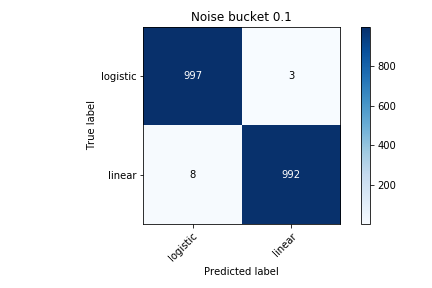
\includegraphics{/Users/andour/Google Drive/projects/Dissertation/Charts/Consusion matrix example 1.png}
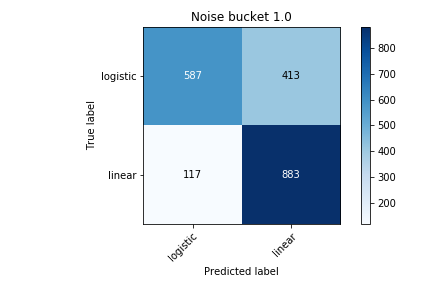
\includegraphics{/Users/andour/Google Drive/projects/Dissertation/Charts/Consusion matrix example 2.png}
This is expected as the signal to noise ratio is very high. However, the
classification clearly becomes less accurate as the noise level
increases. Figures X and Y represent the accuracy and F1 score for
different levels of noise for the frequentist classification approaches:
the accuracy drops quickly after \(\sigma > 0.3\). When the noise
reaches its peak at \(\sigma = 1\) accuracy drops to 0.74 The
frequentist approach although quick to estimate would lead to too many
classification errors.

\begin{figure}
\centering
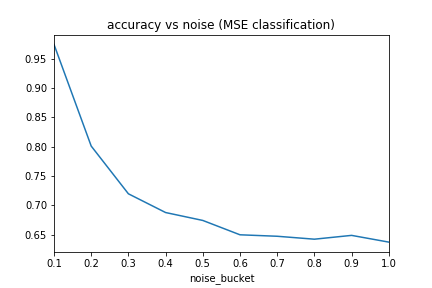
\includegraphics{/Users/andour/Google Drive/projects/Dissertation/plots/accuracy_MSE classification plot.png}
\caption{Caption for the picture.}
\end{figure}

\begin{figure}
\centering
\includegraphics{/Users/andour/Google Drive/projects/Dissertation/plots/F1_MSE classification plot.png}
\caption{Caption for the picture.}
\end{figure}

In terms of parameters, we assume a Gaussian distribution in order to
create parameter confidence intervals {[}TO DO{]}. To analyse this we
observe how the parameter confidence changes as the noise level
increases {[}TO DO{]}\ldots{} Interestingly when observing the behaviour
of the standard deviation of the parameters with regard to noise levels
for the logistic form for instance, \(k\) seems to the slowest variance
change compared to \(L\) and \(x0\).

The MSE method can be contrasted with the BIC evaluation (or Chi square)
which should in theory be more suitable {[}TO DO{]}. Here the results
are \ldots{}

We compare the frequentist methods to the Bayesian classifications
described in section {[}methodology{]}. The first noteworthy point is
that the Bayesian methods were too computationally expensive to run on
the whole dataset. The estimation of one model was about \ldots{} which
would have been \ldots{} for tall the data. This is due to the
computation cost of the MCMC. To still contrast the methodologies, we
sample an even fraction for each noise bucket which we then use as our
sample dataset. The first classification we use is to create a model
based on the median values of each parameter distribution and then
evalute the best model according to the BIC. This simple Bayesian method
yielded surprisingly low classification results : for different levels
of \(\sigma\) the accuracy was always situated between 0.5 and 0.6. This
can be due to the prior settings or the too small number of chains used
in the MCMC process (settings were number chians = \ldots{}, numbe of
burns = \ldots{}).

\begin{figure}
\centering
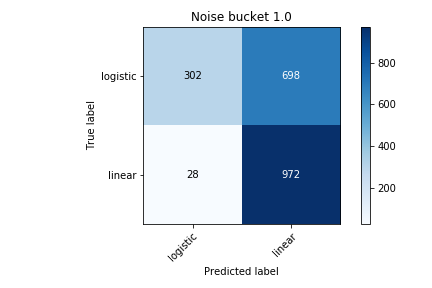
\includegraphics{/Users/andour/Google Drive/projects/Dissertation/plots/Consusion matrix example 2_2.png}
\caption{Caption for the picture.}
\end{figure}

Another possibility can be that the median value is not a good
representative of the parameter distribution. To remedy this we consider
the Bayes factor as our model selection process {[}TO DO{]}. One
advantage of Bayesian modelling is the obtention of parameters as
distribution. This is demonstrated by figure \ldots{}whcih provides an
example of a contour plot for one of the dataset's parameter estimation.

\hypertarget{discussion}{%
\section{Discussion}\label{discussion}}

\hypertarget{evaluation-reflections-and-conclusions}{%
\section{Evaluation, Reflections, and
Conclusions}\label{evaluation-reflections-and-conclusions}}


\end{document}
